% ===================== CHAPTER 11 : APPENDIX =====================
\chapter{APPENDIX}

\section{Sample Code}

\subsection*{Server Entry Point (\texttt{server.js})}

\begin{lstlisting}[language=Java, caption={server.js -- Express.js Application Entry Point}]
require('dotenv').config();
const express  = require('express');
const cors     = require('cors');
const path     = require('path');
const bcrypt   = require('bcryptjs');
const app      = express();

app.use(cors());
app.use(express.json());
app.use(express.urlencoded({ extended: true }));

// Configure session middleware
const session = require('express-session');
app.use(session({
    secret: process.env.SESSION_SECRET || 'tourism_session_secret_2026',
    resave: false,
    saveUninitialized: false,
    cookie: {
        secure: false,
        httpOnly: true,
        maxAge: 7 * 24 * 60 * 60 * 1000 // 7 days
    }
}));

// Route-level protection for dashboard directories
app.use((req, res, next) => {
    const url = req.originalUrl;
    const isDashboard = url.startsWith('/admin')
        || url.startsWith('/user')
        || url.startsWith('/provider');
    if (isDashboard) {
        if (!req.session || !req.session.user) {
            return res.redirect('/login.html?session_expired=true');
        }
        const role = req.session.user.role;
        const rolePaths = {
            admin: '/admin',
            user: '/user',
            provider: '/provider'
        };
        const expectedPrefix = rolePaths[role];
        if (!expectedPrefix || !url.startsWith(expectedPrefix)) {
            return res.redirect(rolePaths[role] + '/');
        }
    }
    next();
});

app.use(express.static(path.join(__dirname, 'public')));

// API Routes
app.use('/api/auth',          require('./routes/auth'));
app.use('/api/destinations',  require('./routes/destinations'));
app.use('/api/bookings',      require('./routes/bookings'));
app.use('/api/services',      require('./routes/services'));
app.use('/api/reviews',       require('./routes/reviews'));
app.use('/api/events',        require('./routes/events'));
app.use('/api/packages',      require('./routes/packages'));
app.use('/api/providers',     require('./routes/providers'));
app.use('/api/notifications', require('./routes/notifications'));
app.use('/api/analytics',     require('./routes/analytics'));
app.use('/api/upload',        require('./routes/uploads'));
app.use('/api/wishlists',     require('./routes/wishlists'));
app.use('/api/payments',      require('./routes/payments'));

const PORT = process.env.PORT || 3000;
app.listen(PORT, () => {
    console.log(`Tourism Marketplace -> http://localhost:${PORT}`);
});
\end{lstlisting}

\subsection*{Authentication Middleware (\texttt{middleware/auth.js})}

\begin{lstlisting}[language=Java, caption={auth.js -- JWT Authentication Middleware}]
const jwt = require('jsonwebtoken');
const SECRET = process.env.JWT_SECRET || 'tourism_promo_secret_2026';

module.exports = function requireAuth(roles = []) {
    return (req, res, next) => {
        const header = req.headers.authorization || '';
        if (!header.startsWith('Bearer ')) {
            return res.status(401).json({
                error: 'Authentication required.'
            });
        }
        const token = header.split(' ')[1];
        try {
            const payload = jwt.verify(token, SECRET);
            if (roles.length && !roles.includes(payload.role)) {
                return res.status(403).json({
                    error: 'Access denied for this role.'
                });
            }
            req.user = payload;
            next();
        } catch {
            return res.status(401).json({
                error: 'Invalid or expired token.'
            });
        }
    };
};
\end{lstlisting}

\subsection*{Database Connection (\texttt{db/connection.js})}

\begin{lstlisting}[language=Java, caption={connection.js -- MySQL Connection Pool}]
const mysql = require('mysql2/promise');

const pool = mysql.createPool({
    host:     process.env.DB_HOST     || 'localhost',
    user:     process.env.DB_USER     || 'root',
    password: process.env.DB_PASSWORD || '',
    database: process.env.DB_NAME     || 'tourism_db',
    waitForConnections: true,
    connectionLimit: 10,
    queueLimit: 0
});

module.exports = pool;
\end{lstlisting}

\subsection*{Database Schema (Excerpt -- \texttt{db/schema.sql})}

\begin{lstlisting}[language=SQL, caption={schema.sql -- Core Table Definitions}]
CREATE DATABASE IF NOT EXISTS tourism_db
    CHARACTER SET utf8mb4
    COLLATE utf8mb4_unicode_ci;
USE tourism_db;

CREATE TABLE IF NOT EXISTS destinations (
    id          VARCHAR(60)   PRIMARY KEY,
    name        VARCHAR(120)  NOT NULL,
    location    VARCHAR(120)  NOT NULL,
    category    VARCHAR(60)   NOT NULL,
    price       INT           NOT NULL DEFAULT 0,
    rating      DECIMAL(3,1)  NOT NULL DEFAULT 4.5,
    image       TEXT,
    description TEXT,
    highlights  TEXT,
    created_at  TIMESTAMP     DEFAULT CURRENT_TIMESTAMP
);

CREATE TABLE IF NOT EXISTS users (
    id          INT           AUTO_INCREMENT PRIMARY KEY,
    name        VARCHAR(120)  NOT NULL,
    email       VARCHAR(120)  UNIQUE NOT NULL,
    password    VARCHAR(255)  NOT NULL,
    role        ENUM('user','admin','provider') DEFAULT 'user',
    created_at  TIMESTAMP     DEFAULT CURRENT_TIMESTAMP
);

CREATE TABLE IF NOT EXISTS bookings (
    id             INT           AUTO_INCREMENT PRIMARY KEY,
    name           VARCHAR(120)  NOT NULL,
    contact        VARCHAR(120)  NOT NULL,
    destination    VARCHAR(120)  NOT NULL,
    package_name   VARCHAR(120)  DEFAULT 'Custom request',
    travel_date    DATE          NOT NULL,
    guests         INT           NOT NULL DEFAULT 1,
    distance_km    DECIMAL(10,2) DEFAULT 0,
    notes          TEXT,
    status         ENUM('Pending','Confirmed','Cancelled')
                   DEFAULT 'Pending',
    created_at     TIMESTAMP     DEFAULT CURRENT_TIMESTAMP
);

CREATE TABLE IF NOT EXISTS reviews (
    id              INT           AUTO_INCREMENT PRIMARY KEY,
    destination_id  VARCHAR(60)   NOT NULL,
    reviewer_name   VARCHAR(120)  NOT NULL,
    rating          TINYINT       NOT NULL DEFAULT 5,
    comment         TEXT,
    created_at      TIMESTAMP     DEFAULT CURRENT_TIMESTAMP
);
\end{lstlisting}

\section{Screenshots}

% Include your actual screenshots here.
% Copy screenshot image files to the report directory
% and uncomment the \includegraphics commands below.

\textbf{Landing Page:}

\begin{figure}[h]
    \centering
    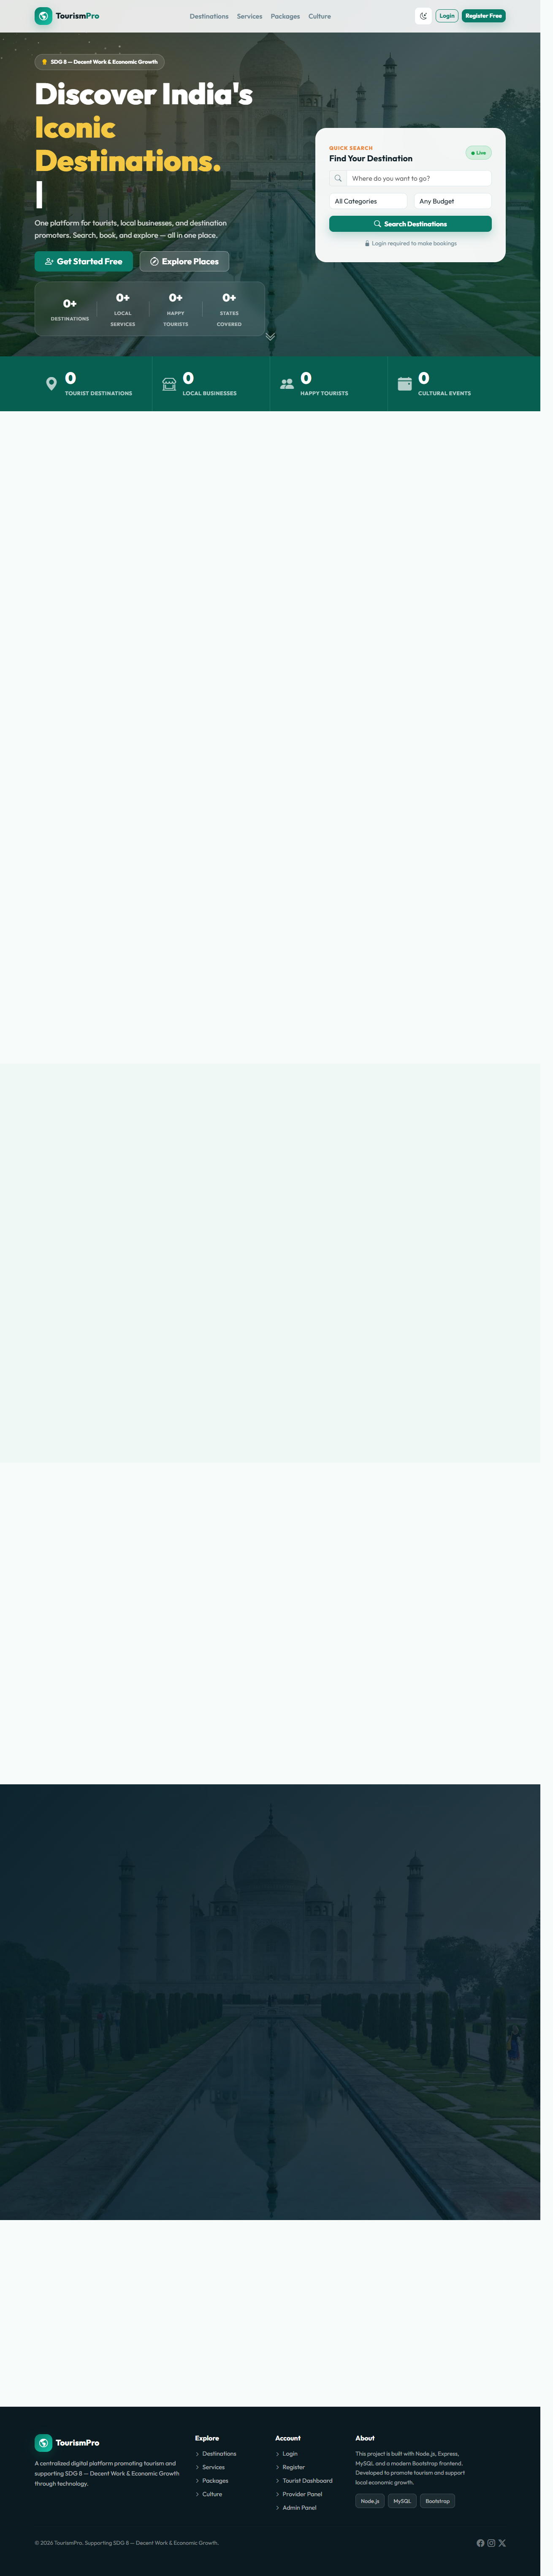
\includegraphics[width=0.95\textwidth]{landing.png}
    \caption{Landing Page -- Tourism Promotion Website}
\end{figure}

\textbf{Registration Page:}

\begin{figure}[h]
    \centering
    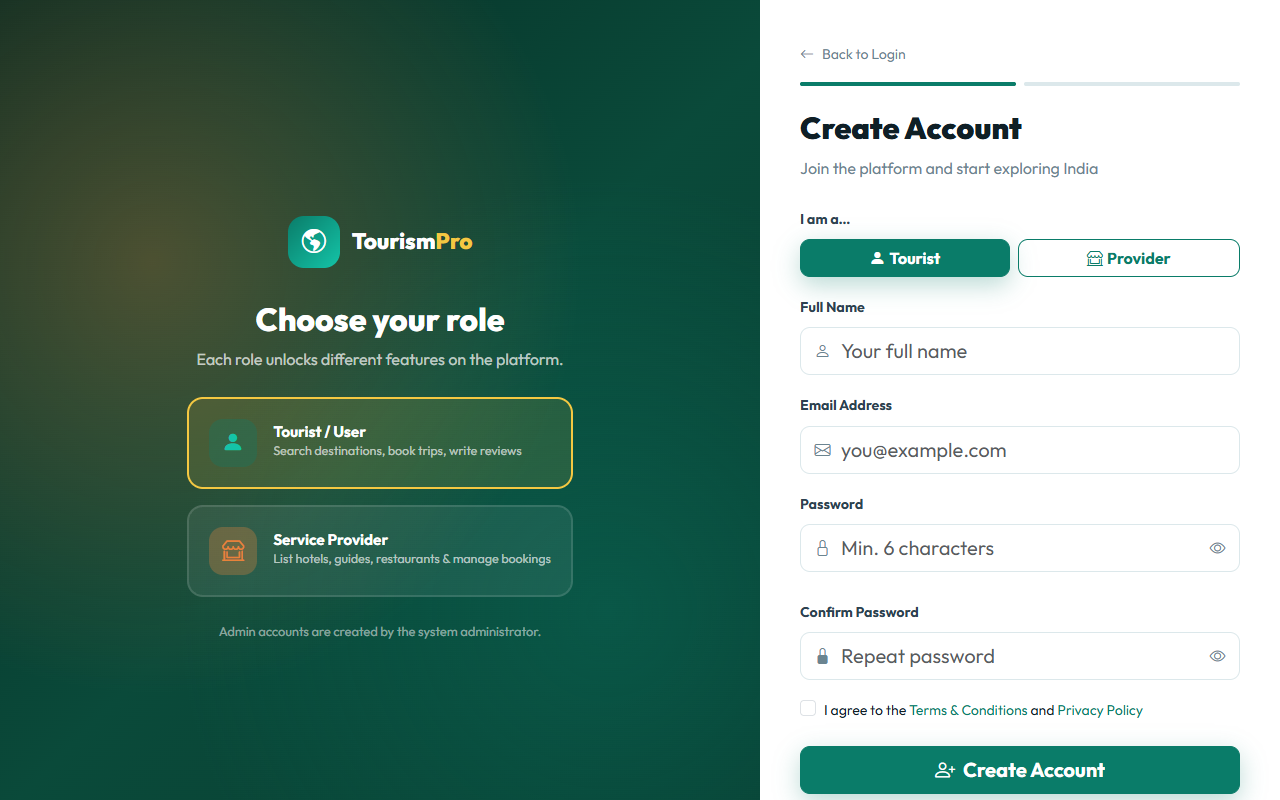
\includegraphics[width=0.95\textwidth]{register.png}
    \caption{User Registration Page}
\end{figure}

% Add more screenshots as needed:
% \begin{figure}[h]
%     \centering
%     \includegraphics[width=0.95\textwidth]{screenshots/login.png}
%     \caption{Login Page}
% \end{figure}
%
% \begin{figure}[h]
%     \centering
%     \includegraphics[width=0.95\textwidth]{screenshots/admin_dashboard.png}
%     \caption{Admin Dashboard}
% \end{figure}
%
% \begin{figure}[h]
%     \centering
%     \includegraphics[width=0.95\textwidth]{screenshots/provider_dashboard.png}
%     \caption{Service Provider Dashboard}
% \end{figure}
%
% \begin{figure}[h]
%     \centering
%     \includegraphics[width=0.95\textwidth]{screenshots/user_dashboard.png}
%     \caption{Tourist Dashboard}
% \end{figure}
%
% \begin{figure}[h]
%     \centering
%     \includegraphics[width=0.95\textwidth]{screenshots/destination_detail.png}
%     \caption{Destination Detail Page}
% \end{figure}

\section{Git Logs}

% If you have a Git repository, paste your git log output here.
% Run: git log --oneline --graph --all
% and paste the output between \begin{verbatim} and \end{verbatim}

\begin{verbatim}
commit  - Initial project setup with Express.js and MySQL
commit  - Database schema with destinations, services,
          packages, events, bookings, and reviews
commit  - Authentication system with JWT and bcrypt
commit  - Destination CRUD API routes
commit  - Booking management API
commit  - Service listing and provider API
commit  - Landing page with Bootstrap 5 and AOS animations
commit  - Login and registration pages with role selection
commit  - Admin dashboard with user and content management
commit  - Tourist dashboard with bookings and wishlists
commit  - Provider dashboard with service management
commit  - Payment processing module
commit  - Notification system implementation
commit  - Analytics dashboard for admin
commit  - Database migration v2 with extended tables
commit  - Provider approval workflow
commit  - Dark/light theme toggle
commit  - Responsive design improvements
commit  - Final testing and bug fixes
commit  - Documentation and project report
\end{verbatim}

% To generate actual git logs, run the following command
% in your project directory and replace the above:
%   git log --oneline -20
